\documentclass[a4paper,10pt]{article}
\usepackage{graphicx,color}
\usepackage[margin=2cm]{geometry}
\usepackage{algorithm2e}

\begin{document}

{\LARGE{\centerline{\bf Lab 1}}}

\section{3-D Array Multiplication}

To obtain each element in matrix $C$, matrix $A$ and $B$ are divided into two dimensional matrices, $A'$ and $B'$ as can be seen in figure \ref{3DMult}.
For each two dimensional matrix, a single row and column is multiplied to get the corresonding element in the $C$ matrix.
This leads to a single value which is the element in the $C$ matrix.
This is done for all elements in the $C$ matrix.

\begin{figure}[h]
\centering
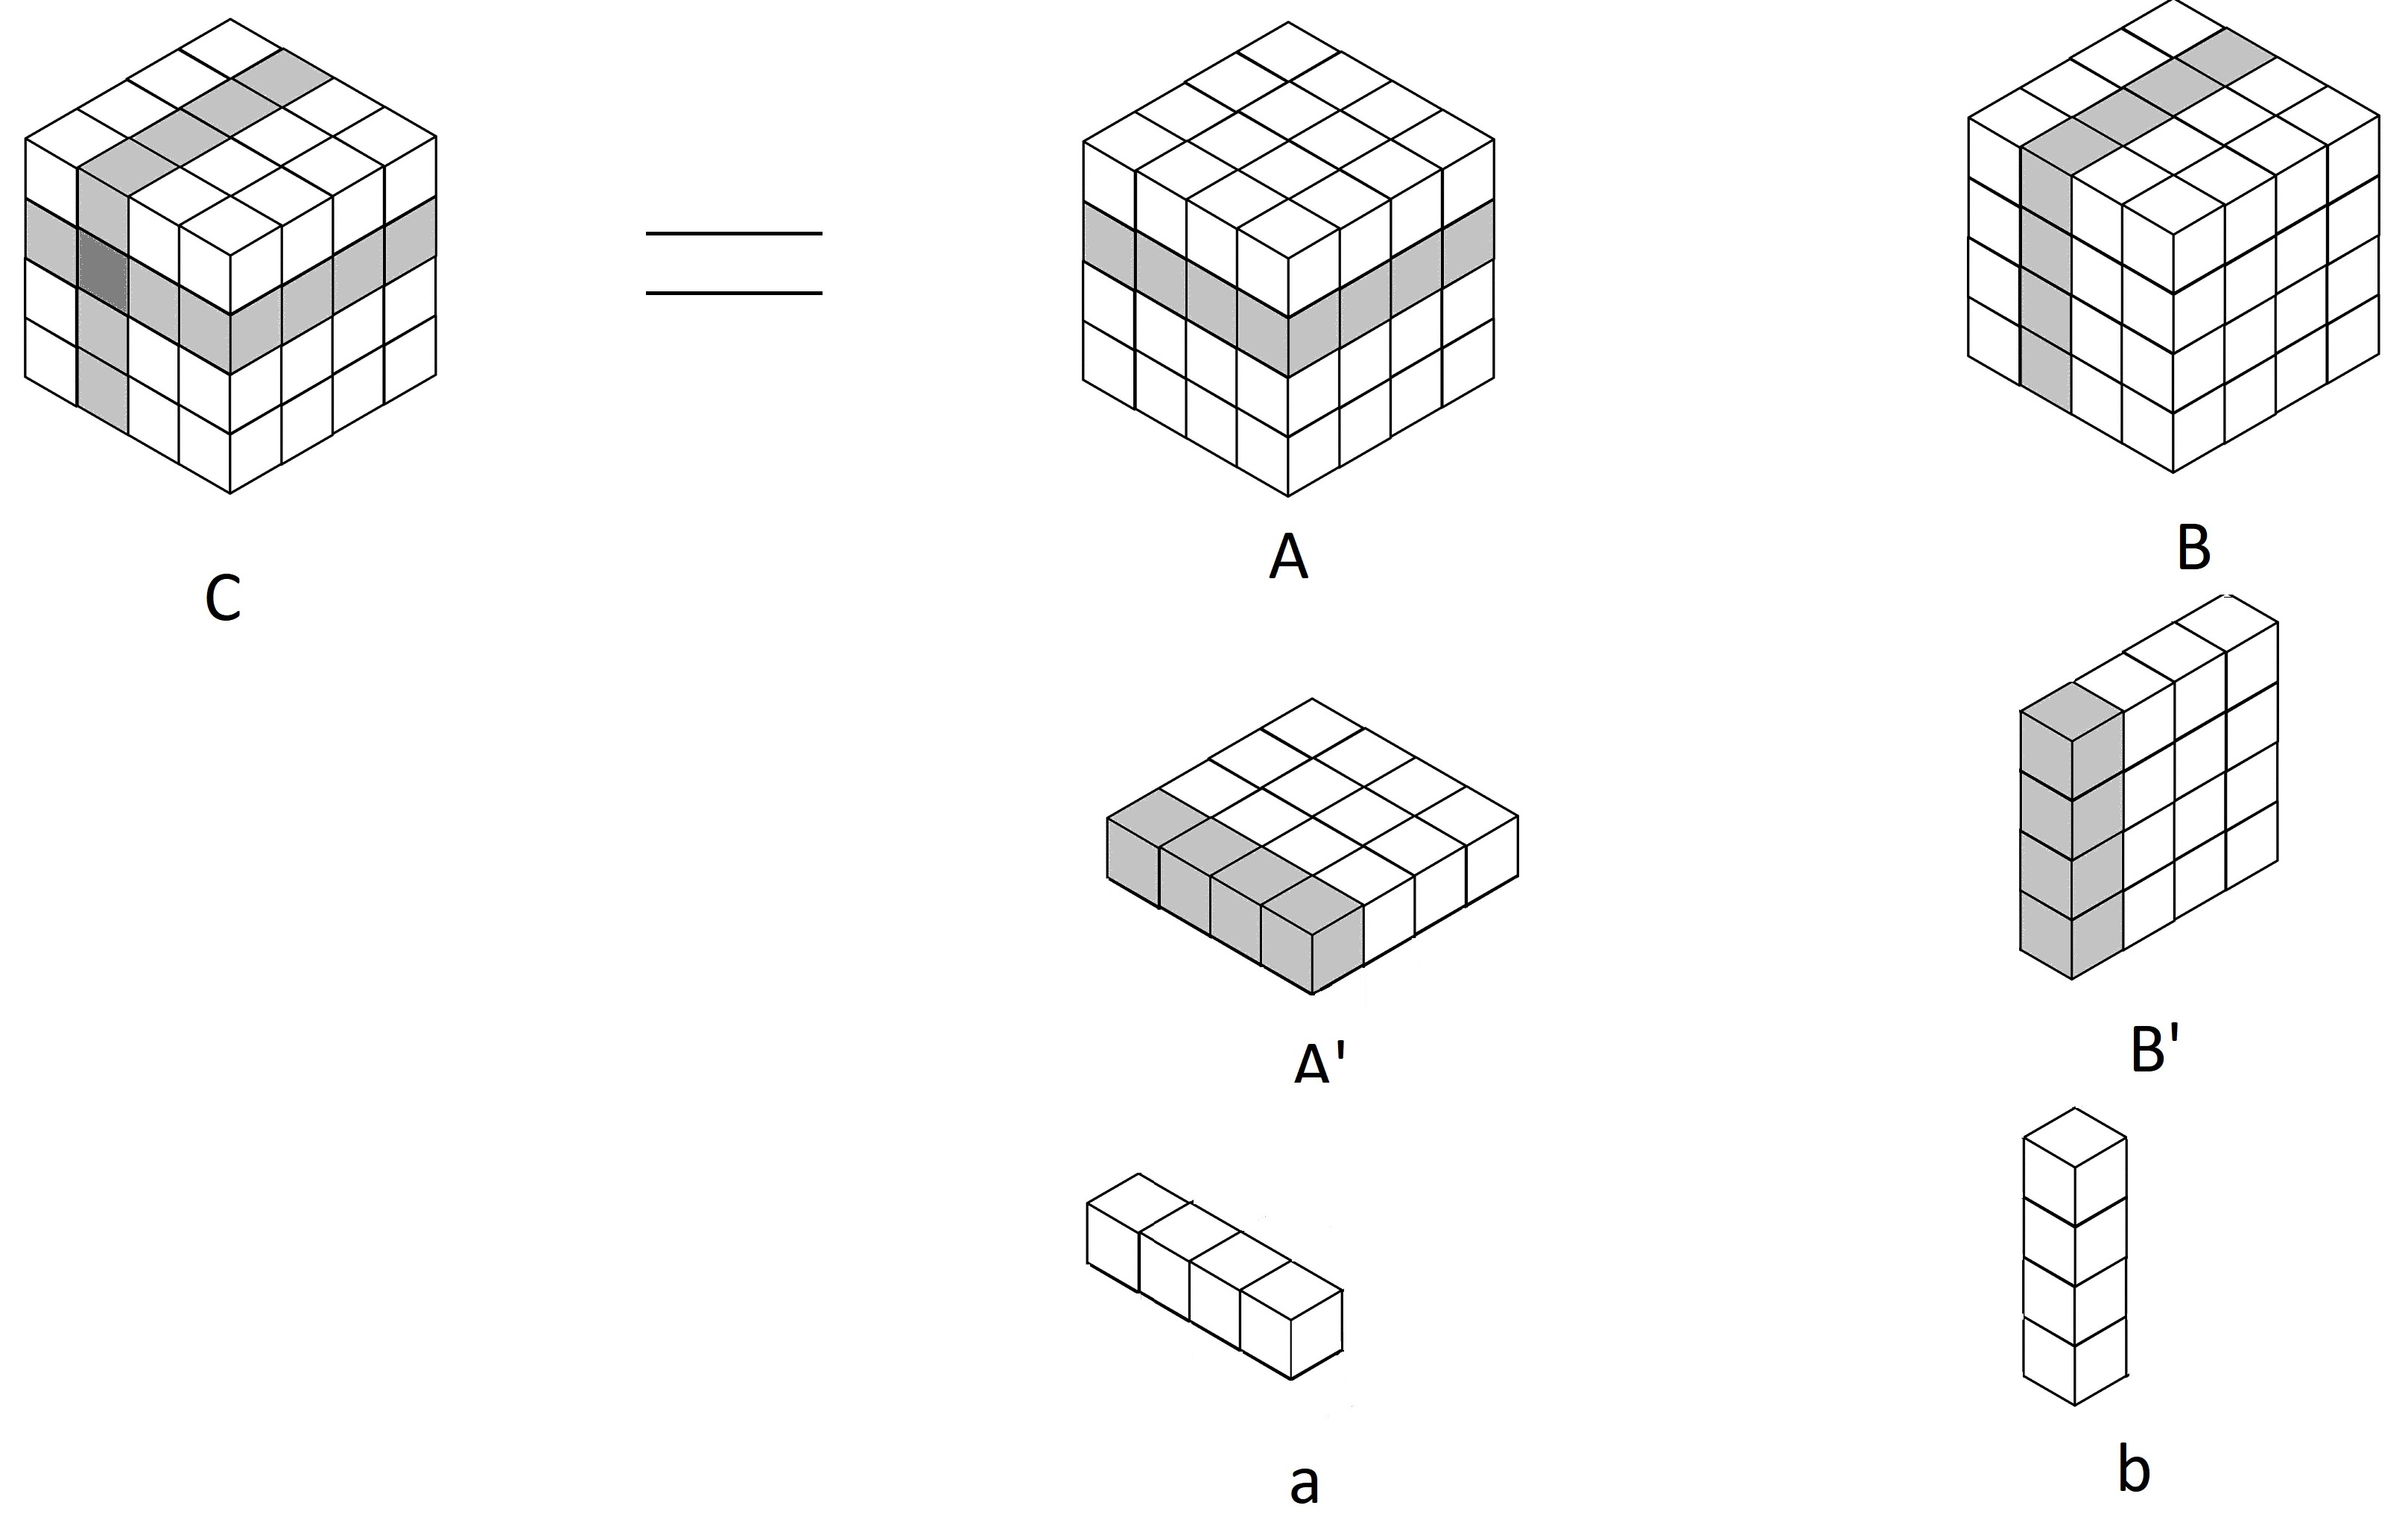
\includegraphics[scale=0.15]{3D.jpg}
\caption{How each element in $C$ was obtained from matrices $A$ and $B$.}\label{3DMult}
\end{figure}

Two \texttt{for} loops were used to maintain the row and column of the current element in matrix $C$.
Another \texttt{for} loop was used to traverse the depth of the matrix $C$.
The row $a$ and column $b$ were then obtained from matrices $A$ and $B$ as seen in figure \ref{3DMult}.
Vector multiplication was then used on vectors $a$ and $b$.
The resulting value is the corresponding element of $C$.

This was repeated for all elements in matrix $C$.
It was assumed matrix $A$ and $B$ are cubes.

\section{Pseudocode}

\begin{algorithm}[H]
\SetAlgoLined
\SetKwData{Left}{left}\SetKwData{This}{this}\SetKwData{Up}{up}
\SetKwFunction{Union}{Union}\SetKwFunction{FindCompress}{FindCompress}
\SetKwInOut{Input}{input}\SetKwInOut{Output}{output}
\Input{Matrix A and B}
\Output{Matrix C }
\BlankLine
\For{each row in matrix C}{
\For{each column in matrix C}{\label{forins}
\For{each depth in matrix C}{
Get corresponding row at depth from matrix A\;
Get corresponding column at depth from matrix B\;
Multiply the obtained row and column to get the value of matrix C at the current row, column and depth.
}}}
\caption{rank3TensorMult pseudocode}\label{algo_disjdecomp}

\end{algorithm}

\end{document}